\documentclass[preprint,12pt]{elsarticle}
\usepackage[utf8]{inputenc}
\usepackage[T1]{fontenc}
\usepackage{amsmath,amssymb,graphicx,booktabs,tabularx,array}
\usepackage[margin=25mm]{geometry}
\usepackage{url}
\journal{Sensors and Actuators A: Physical}
\begin{document}
\begin{frontmatter}
\title{Supplementary methods and provenance for five node magnetic contact reconstruction}
\author{[Author names and affiliations to be inserted]}
\end{frontmatter}
\section{S1 Experimental identities and scientific names}

CCA is the concentric alternating-polarity disc array, internally labelled 19C. CPA is the checkerboard alternating-polarity disc array, internally labelled 5x5. PSM-L and PSM-H are parallel-stripe magnetic sheets with nominal isolation layers of 2.5 and 4.5 mm, internally labelled flot1650-2.5mm and flot1650-4.5mm. They are three layouts and four configurations. The historical indenter label flat\_d6mm denotes mounting-related metadata, not the contacting diameter. The confirmed contact-end diameter is 1 mm; the outer dimension is 4 mm and the mounting thread is M6 \ensuremath{\times} 1.

SC-RBF denotes sparse-calibration continuous regression, DC-RBF dense-calibration continuous regression, WD-RBF working-domain regression, DPL discrete prototype localization, and WD-Causal a working-domain kernel decoder with causal history correction. Names alone do not identify a training set. The model file and the table below together define the evaluated instance.

\begin{center}\small
\begin{tabularx}{\linewidth}{>{\raggedright\arraybackslash}X>{\raggedright\arraybackslash}X>{\raggedright\arraybackslash}X>{\raggedright\arraybackslash}X}
\toprule
Evaluation & Training source & Test source & Interpretation \\
\midrule
Four configurations & S20260917\_A plans; 36 of 121 positions & Other 85 positions, 510 contacts per configuration & Spatial generalization \\
Frozen CPA SC-RBF and DC-RBF & S20260918\_A Trials 149, 150, 153 & Trial 154; 441 contacts & Independent repeated contacts at known grid positions \\
DPL & Historical mixed pool; 2489 contacts & The same reserved Trial 154 & Discrete-node task, not a controlled training-density comparison \\
WD-RBF cross scan & Same-source deployment using 0.4 and 0.6 mm & S20260920\_A Trial 005 & Later motion record \\
WD-Causal radial and circle & Earlier CPA static source plus nine earlier motion records & S20260920\_A Trials 017, 018, 020 & New trajectory recordings \\
Dense deployment XYZ & Historical mixed pool, 2489 contacts & S20260920\_A Trials 026, 030, 032, 036 & New simultaneous XYZ motion \\
\bottomrule
\end{tabularx}\end{center}

Table S1. Dataset roles. Some later production models include Trial 154; they must not replace the frozen models when reproducing the independent static result.

The matched four-configuration source plans end in 202428 for CCA, 211757 for CPA, 143129 for PSM-L and 220949 for PSM-H on 17 September 2026. The frozen CCA comparison is not replaced by a later remounted CCA model. Exact plan names are preserved in the data files. Each configuration provides 121 positions \ensuremath{\times} three depths \ensuremath{\times} two repeats = 726 contacts. Spatial parameter selection and the 85-location evaluation are separate from the subsequent full-map deployment fit.

\section{S2 Model implementation details}

The frozen static reproduction script rebuilds both continuous models from contact-level delta-B values and checks them against the saved coefficient arrays. The sparse training set contains 363 contacts and the dense set 1322 contacts. Both predict all 441 reserved contacts without a contact gate. Their exact planar mean errors are 0.349466985 and 0.288394377 mm. The dense per-axis MAEs are 0.163168897, 0.205812498 and 0.031477144 mm. DPL identifies 412 nodes correctly and has planar mean error 0.073112564 mm and Z MAE 0.010700187 mm.

For DPL, the score of a position is the maximum cosine similarity over its template bank, not the cosine similarity to a single averaged template. If A = kz + b is the local fitted amplitude relation, the decoded indentation is (A - b)/max(k, epsilon). DPL uses an additional historical source pool and is not used to attribute improvement solely to model type.

The frozen dense regression uses 441 unit-response centres, a 441 \ensuremath{\times} 2 XY coefficient matrix and 33 depth coefficients including the last-column intercept. The sparse depth feature concatenates raw delta-B, log amplitude and squared log amplitude. Scales below 10 to the power -6 are replaced by one. The released offline predictor checks input shape and finiteness and reproduces the reference predictions.

The selected WD-Causal model uses a standardized Gaussian kernel of the form exp(-gamma \ensuremath{\times} squared distance / bandwidth). XY parameters are gamma = 0.1, ridge penalty = 0.001 and bandwidth = 59.5226290521. Z parameters are gamma = 0.3, ridge penalty = 0.01 and bandwidth = 0.586188748. The Z output mean is 0.65 mm. Training coordinates, standardization and output means are retained with the model. The base XY feature is the 32-dimensional shape--log-amplitude interaction feature; the base Z feature is the 15-dimensional raw difference.

For the history gate, the instantaneous activation is clipped to the interval zero to one after computing the normalized short-lag magnetic-change magnitude divided by 0.0267405688 minus one. The current gate is the larger of this activation and the preceding gate multiplied by exp(-dt/1.2 s). A gap above 0.25 s resets history. The residual model has 136 standardized features and a first-column intercept, giving 137 \ensuremath{\times} 3 coefficients. The intercept convention therefore differs from the frozen static depth model. Its nine dynamic training records are S20260918\_A Plan\_20260918\_022707 Trials 078--085 and 090. None of the reported S20260920\_A radial or circle records participates in this training.

\section{S3 Dynamic records and selection}

The public dynamic export contains 39 records and their disposition, parameters, mounting calibration, segment predictions, references and validity counts. Numerical reproduction recalculates 236 scalar checks from those arrays. This verifies the recorded-output metrics; it is not a new inference run from the original magnetic streams.

Trial 001 is aborted. Trials 002, 003, 006, 007 and 008 are raw-fingerprint calibration comparison records. Trials 012 and 014 have invalid initialization and are excluded from main performance evaluation. The other 31 records remain in the audit and are interpreted according to their model and condition. Poor coverage in Trials 027, 029 and 033 is retained as an operating-boundary result, not silently attributed to initialization. These trials have approximately 62.4\%, 36.5\% and 50.7\% coverage, predominantly due to template-similarity rejection.

\begin{center}\small
\begin{tabularx}{\linewidth}{>{\raggedright\arraybackslash}X>{\raggedright\arraybackslash}X>{\raggedright\arraybackslash}X>{\raggedright\arraybackslash}X>{\raggedright\arraybackslash}X}
\toprule
Trial in S20260920\_A & Condition & Planar error mm & Z MAE mm & Coverage \\
\midrule
004 & SC-RBF cross, extent 6 mm & 0.855 & 0.0498 & 100\% \\
005 & WD-RBF cross, extent 6 mm & 0.510 & 0.0789 & 97.44\% \\
017 & WD-Causal eight directions, radius 4 mm & 0.453 & 0.0556 & 100\% \\
018 & WD-Causal circle, radius 2 mm, movement only & 0.407 & 0.0485 & 100\% \\
020 & WD-Causal circle, radius 4 mm, movement only & 0.772 & 0.0829 & 100\% \\
026 & XYZ increment (-4, +4, +1.2) mm & 0.613 & 0.1012 & 100\% \\
030 & XYZ increment (-8, +8, +1.4) mm & 0.679 & 0.1134 & 100\% \\
032 & XYZ increment (+8, -8, +1.2) mm & 0.561 & 0.0725 & 99.91\% \\
036 & XYZ increment (-6, +6, +1.0) mm & 0.570 & 0.1042 & 100\% \\
039 & Later static 81-position grid at 0.6 mm & 0.728 & 0.1063 & 100\% \\
\bottomrule
\end{tabularx}\end{center}

Table S2. Record-level results, with static Trial 039 evaluated on final hold medians rather than motion frames. It is a later-session result and is not substituted for the reserved static result in the abstract.

Trial 032 contains 550 and 541 valid samples in its two executions. Their XYZ mean errors are 0.564253 and 0.573692 mm. The saved mounting transform for Trials 026--039 is a planar rotation of -5.3205175 degrees and translation (1.5632454, 0.9619818) mm. The transform for Trials 015--025 is -10.4907044 degrees with translation (2.3352261, 0.7579724) mm. These are recorded pre-test calibration states, not transforms fitted to the test paths. Different model and calibration states mean that Trial 025 versus Trial 026 is not a clean paired algorithm ablation.

Circular movement is generated as 128 linear segments with host waiting. Full-contact errors, including waits, are 0.3904056 and 0.7518913 mm for WD-Causal radii of 2 and 4 mm. Average complete-path speeds are approximately 0.322351 and 0.555654 mm/s. No fitted-circle correction is used to compute these absolute errors. Coverage includes eligible samples in segments that contain no valid predictions.

\section{S4 Physical documentation and videos}

\begin{center}
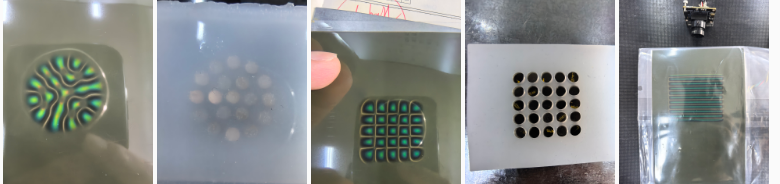
\includegraphics[width=\linewidth,height=.47\textheight,keepaspectratio]{assets/magnetic_layers_and_viewing_film.png}
\end{center}

Figure S1. Supplied photographs, from left to right, show the CCA viewing-film pattern, CCA specimen, CPA viewing-film pattern, CPA arrangement and PSM viewing-film pattern. Viewing-film contrast is qualitative evidence of magnetic organization, not a calibrated field-magnitude map.

\begin{center}
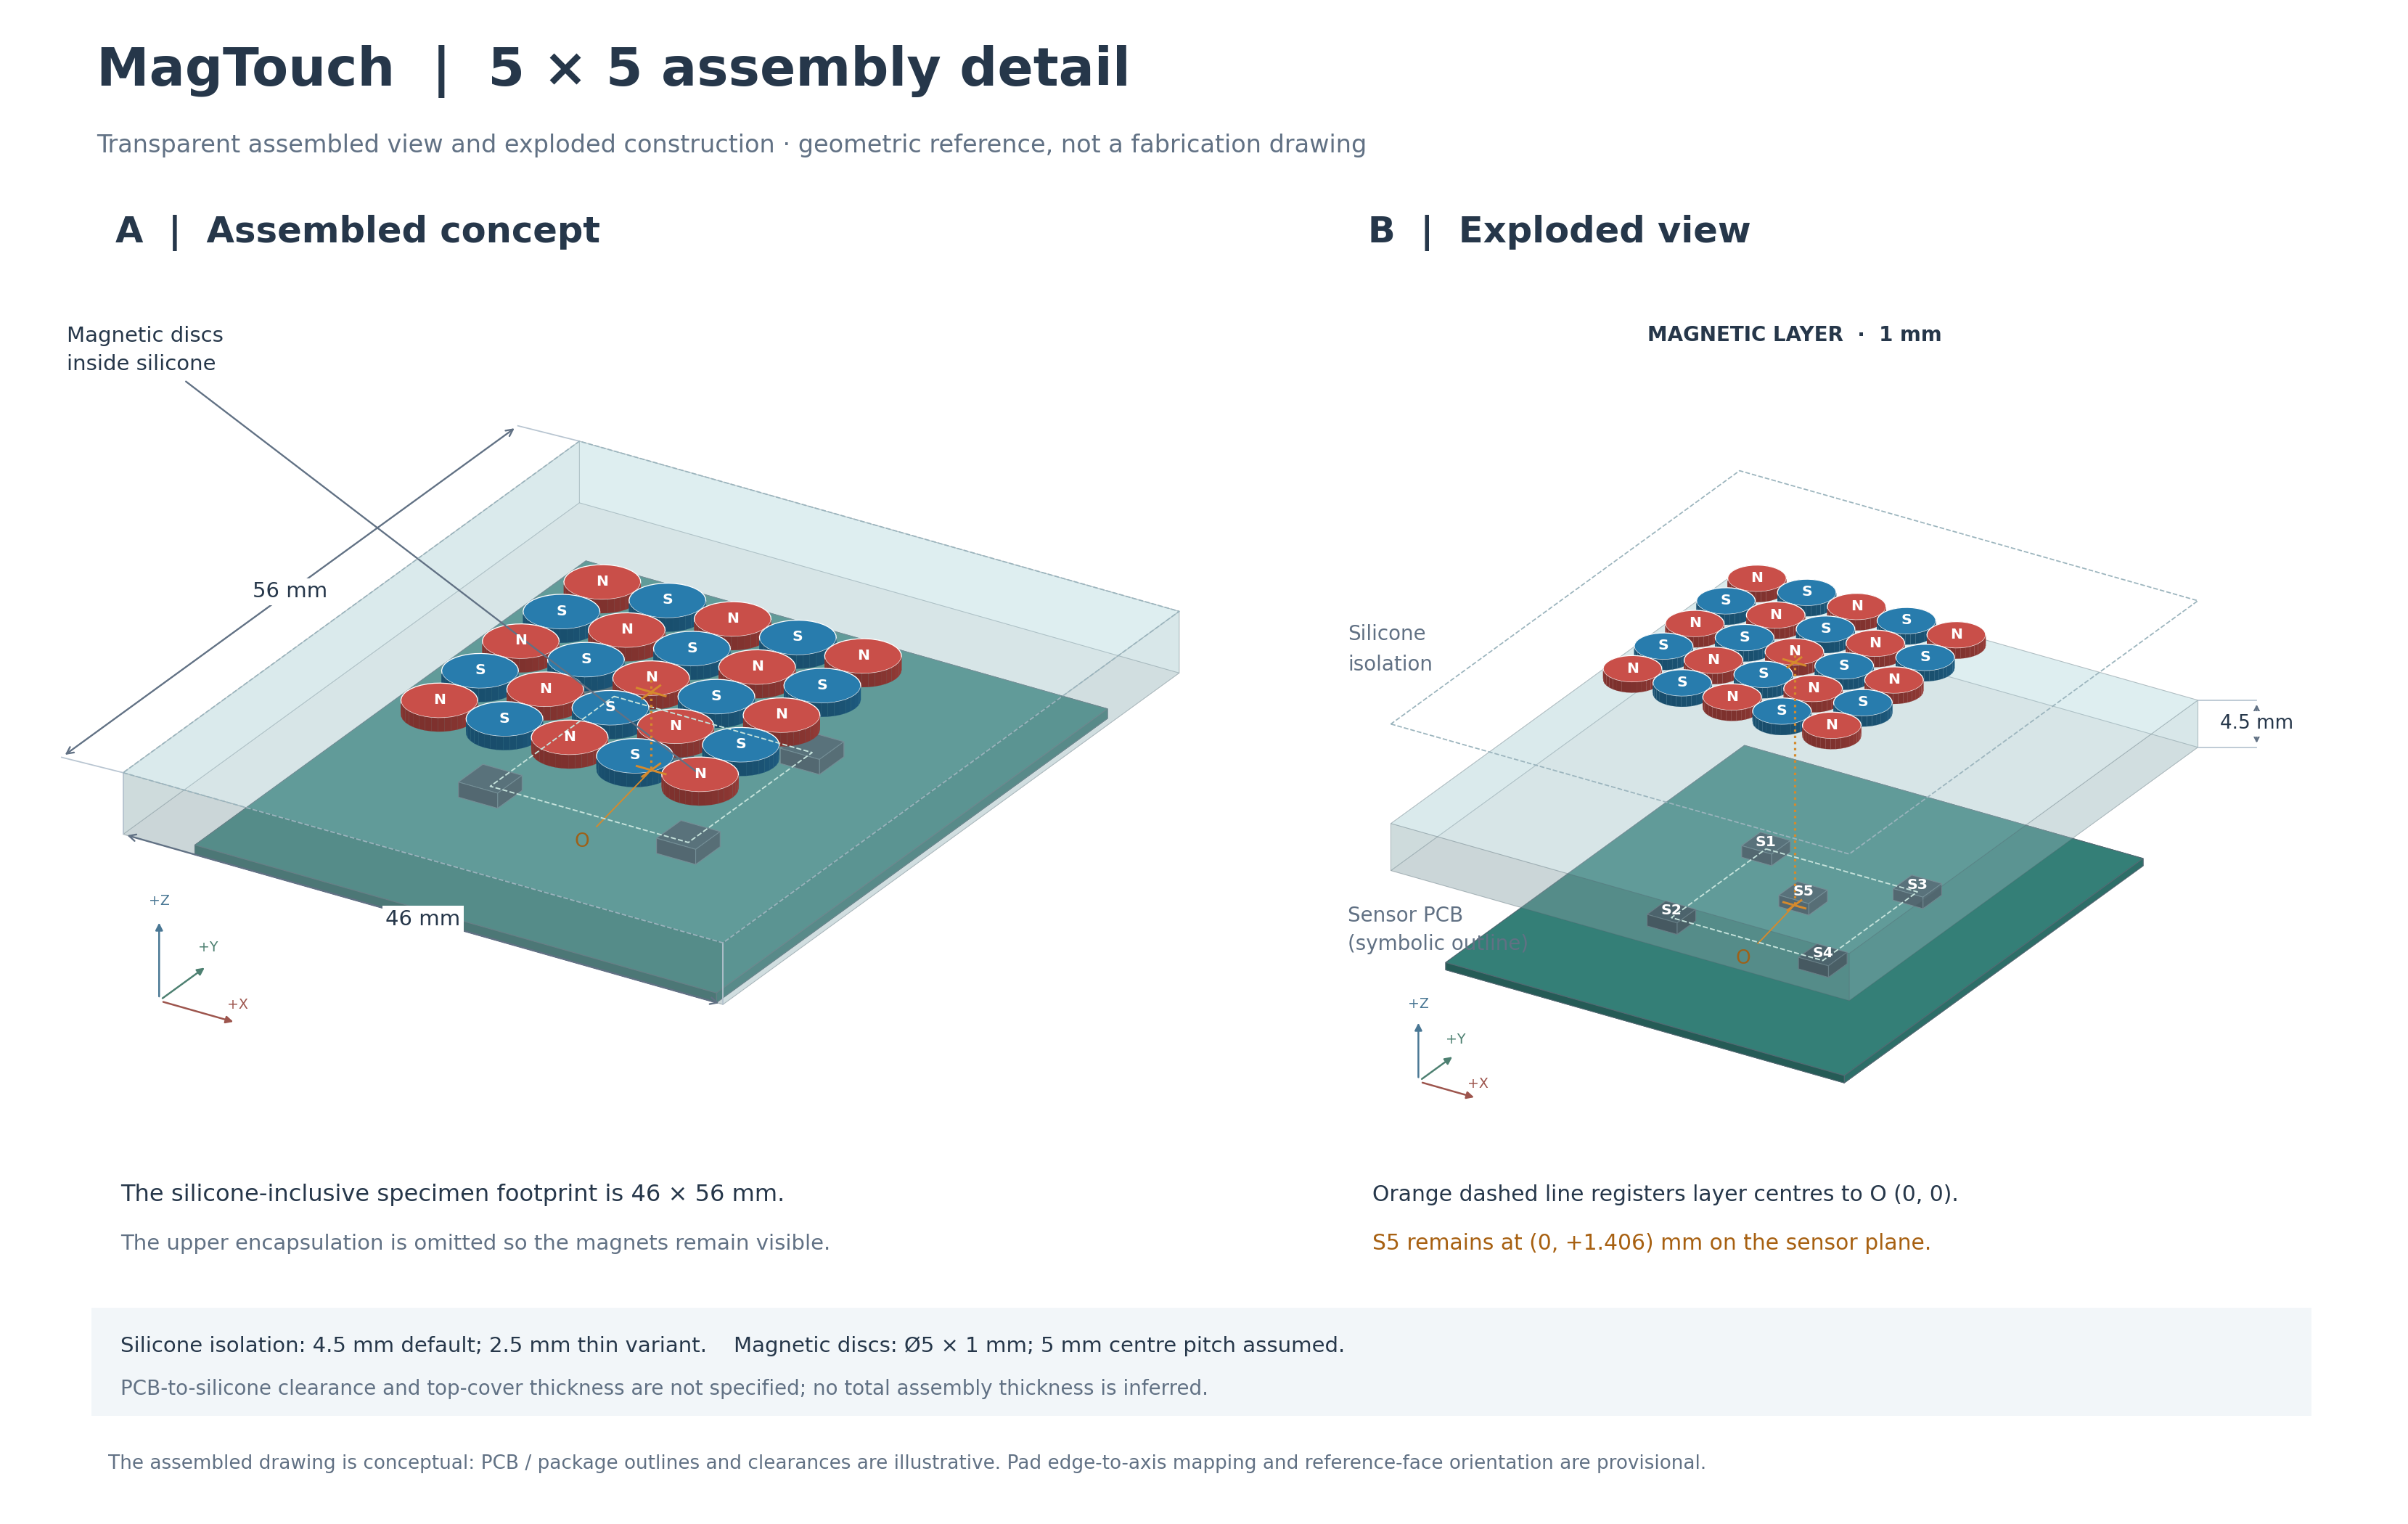
\includegraphics[width=\linewidth,height=.47\textheight,keepaspectratio]{assets/assembly.png}
\end{center}

Figure S2. Existing assembled and exploded drawing of the checkerboard specimen. The gaps in the exploded view are illustrative. The drawing is a structural model, not a field simulation or a deformation solution.

Video S1 shows a replay of recorded cross-scan measurements from S20260919\_A Trial 035, together with the side-view camera and recorded model trajectory. Video S2 shows a replay segment of S20260920\_A Trial 036, with simultaneous XYZ motion, recorded camera images and reconstructed coordinates. These are recordings of the replay interface displaying real experimental data; they are not labelled as fresh live acquisition videos. Their filenames preserve the originally supplied clips. No new experimental frames are generated.

\section{S5 Reproducibility and remaining submission metadata}

The repository separates static contact-level reproduction, dynamic recorded-output reproduction, model parameters, specimen documentation and the manuscript. The compact static export supports refitting the frozen continuous models. The dynamic export supports checking errors and coverage but does not include all raw 15-channel magnetic streams or every acquisition command needed to regenerate the entire acquisition pipeline. Original full records are retained locally.

Author names, affiliations, funding and declarations remain placeholders by request. Silicone formulation, curing conditions and hardness must be confirmed from fabrication records before submission. Journal-specific upload requirements must be checked in the submission system. No manuscript has been submitted and no repository content has been pushed as part of preparing this package.

\end{document}